\chapter{Supplementary information}
\label{app:supp}

\section{Unmarked figures}
\label{sec:unmarked}

\subsection{January means for selected variables 1 (unmarked)}

The use of coloured markings with thick outline in Figure~\ref{fig:wa_jan_comb_1} somewhat distorts perception of the trends. For an undistorted view, see Figure~\ref{fig:wa_jan_comb_1_unmarked}.

\begin{figure}[!htp]
	\centering
	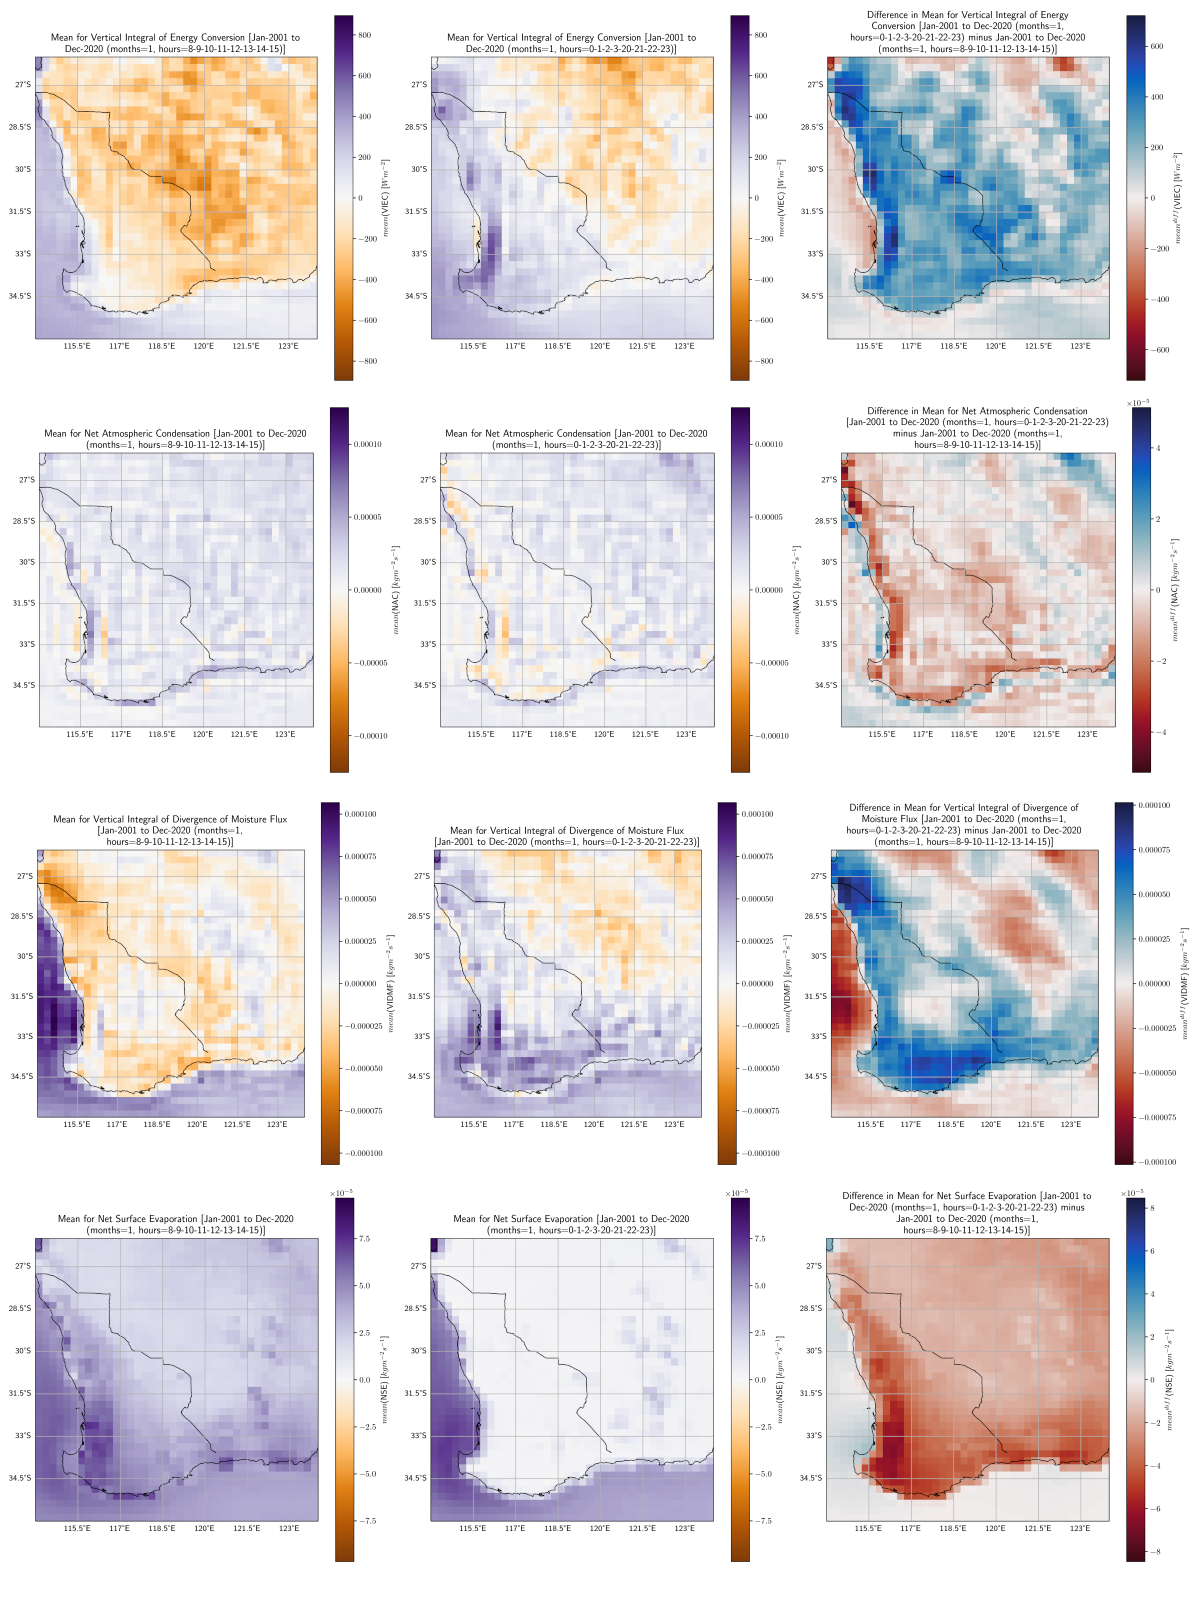
\includegraphics[width=0.9\textwidth]{wa_jan_comb_1_unmarked.png}
	\caption[January means for selected variables 1 (unmarked)]{January mean daytime and nighttime values for \acs{VIEC}, \acs{NAC}, \acs{VIDMF} and \acs{NSE}.}
	\label{fig:wa_jan_comb_1_unmarked}
\end{figure}

\subsection{January means for selected variables 2 (unmarked)}

The use of coloured markings with thick outline in Figure~\ref{fig:wa_jan_comb_2} somewhat distorts perception of the trends. For an undistorted view, see Figure~\ref{fig:wa_jan_comb_2_unmarked}.

\begin{figure}[!htp]
	\centering
	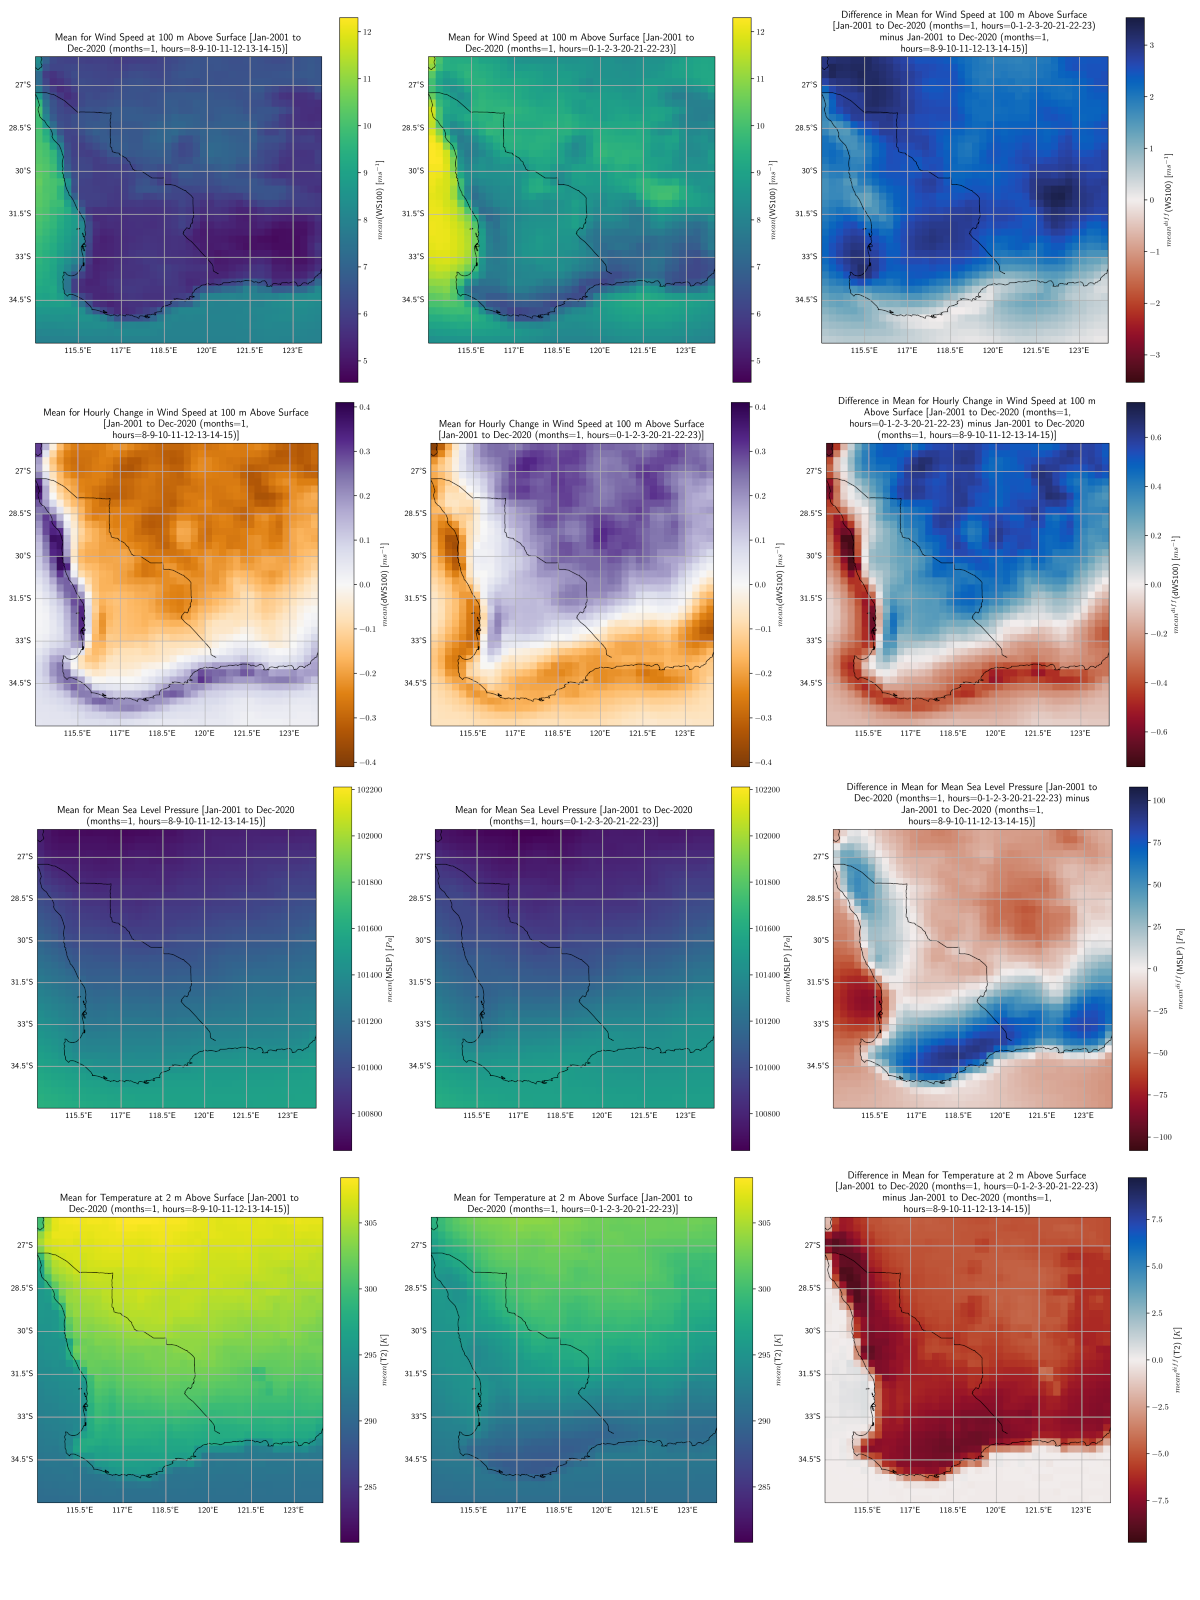
\includegraphics[width=0.9\textwidth]{wa_jan_comb_2_unmarked.png}
	\caption[January means for selected variables 2 (unmarked)]{January mean daytime and nighttime values for \acs{WS100}, \acs{dWS100}, \acs{MSLP} and \acs{T2}.}
	\label{fig:wa_jan_comb_2_unmarked}
\end{figure}

\section{Similar comparison results}
\label{sec:results_sim}

\subsection{Selected MDP means for similar comparison}

See Figure~\ref{fig:wa_stats_similiar_1} for \ac{MDP} means results discussed in Section~\ref{ssec:similar_find}.

\begin{figure}[!htp]
	\centering
	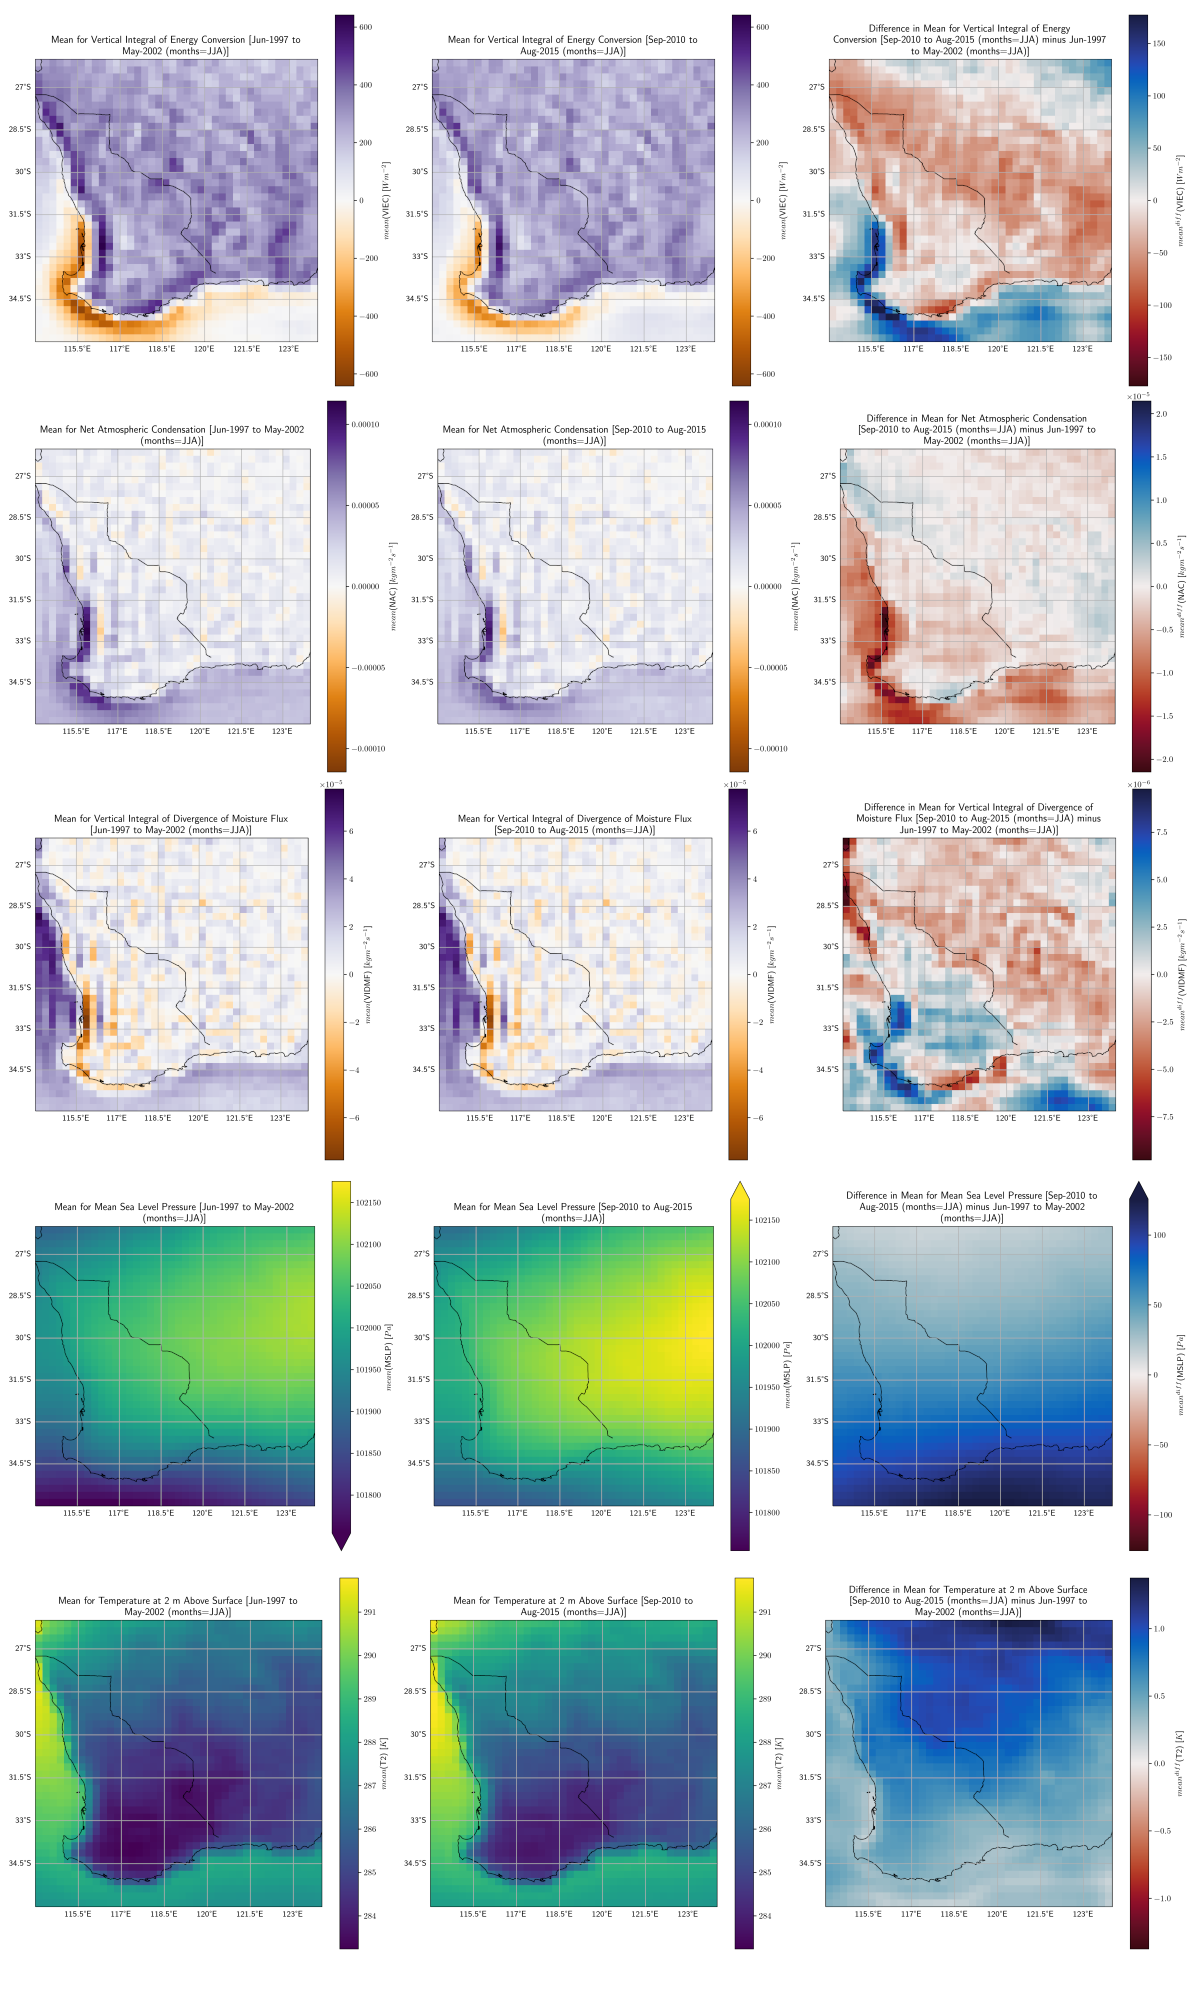
\includegraphics[width=0.75\textwidth]{wa_stats_similar_1.png}
	\caption[Selected MDP means for similar comparison]{Selected \ac{MDP} means (across various variables) for similar comparison which displayed delineations along the fence. Top to bottom: $mean$(\acs{VIEC}), $mean$(\acs{NAC}), $mean$(\acs{VIDMF}), $mean$(\acs{MSLP}), $mean$(\acs{T2}).}
	\label{fig:wa_stats_similiar_1}
\end{figure}

\subsection{Selected MDP stats for similar comparison}

See Figure~\ref{fig:wa_stats_similiar_2} for \ac{MDP} statistics results discussed in Section~\ref{ssec:similar_find}.

\begin{figure}[!htp]
	\centering
	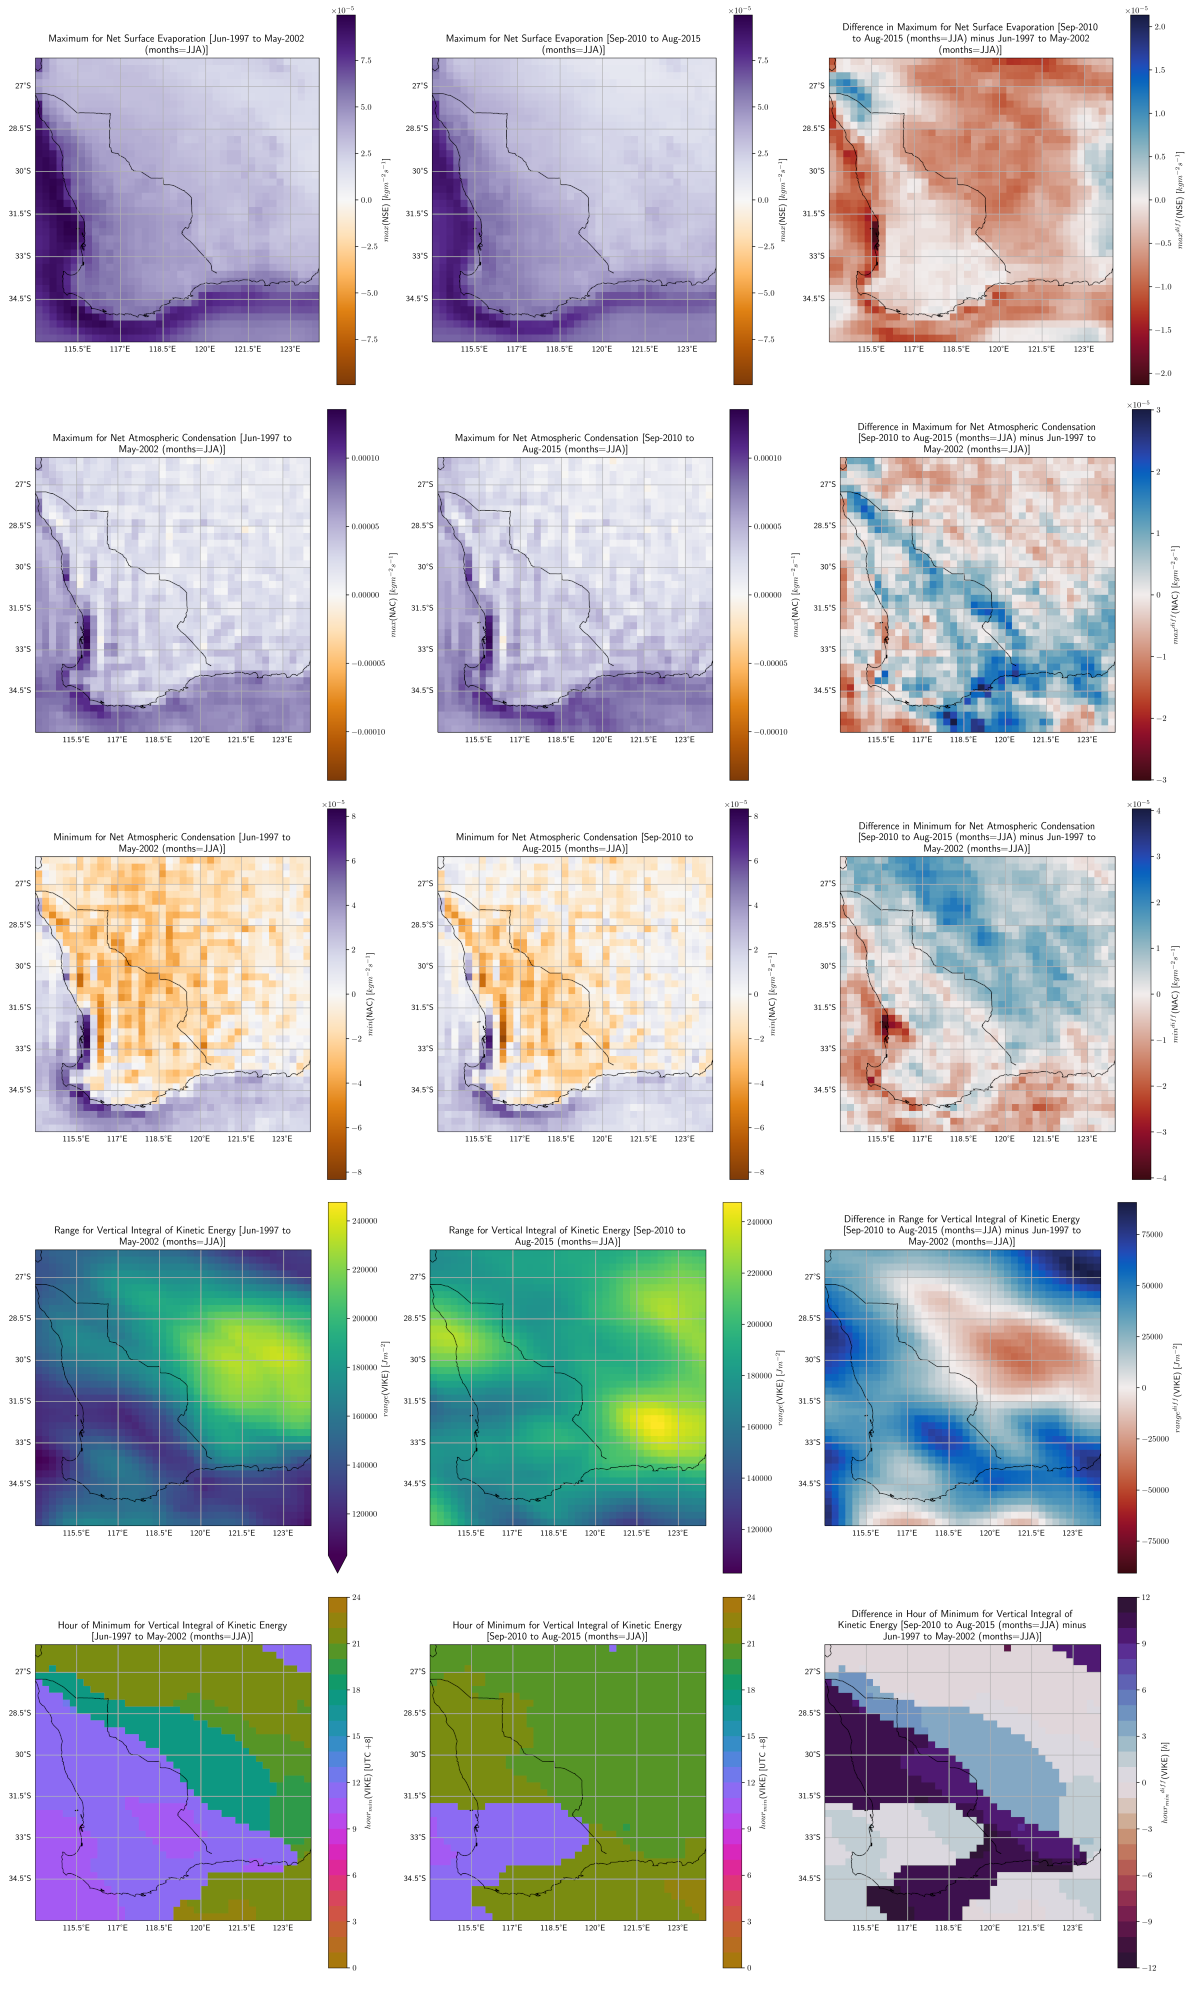
\includegraphics[width=0.75\textwidth]{wa_stats_similar_2.png}
	\caption[Selected MDP stats for similar comparison]{Selected \ac{MDP} statistics (across various variables) for similar comparison which displayed delineations along the fence. Top to bottom: $max^{diff}$(\acs{NSE}), $max^{diff}$(\acs{NAC}), $min^{diff}$(\acs{NAC}), $range$(\acs{VIKE}), $hour_{min}$(\acs{VIKE}). Note that \ac{NAC} stats have artefacts (see Appendix~\ref{sec:artefact}).}
	\label{fig:wa_stats_similiar_2}
\end{figure}

\begin{figure}[!htp]
	\centering
	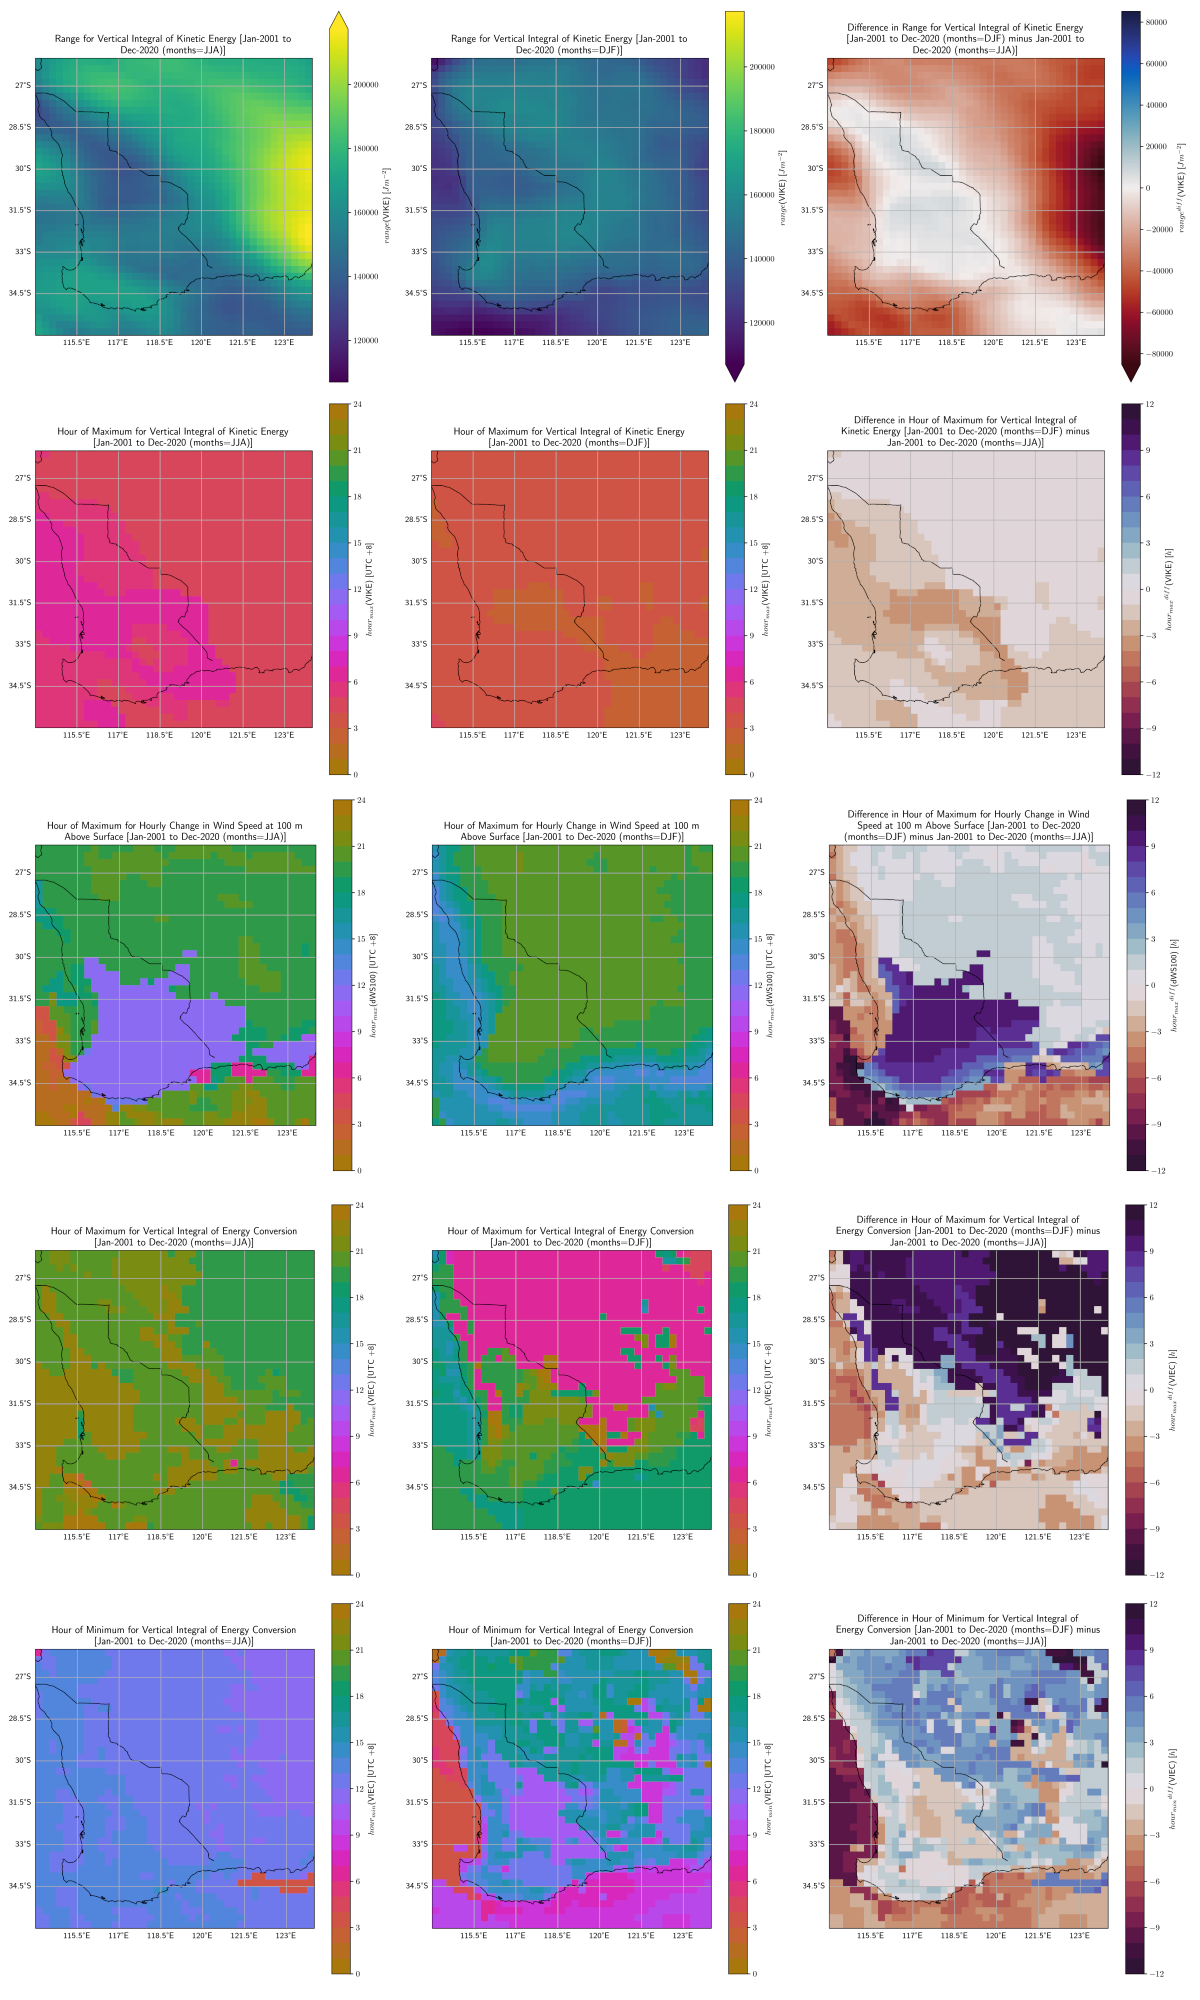
\includegraphics[width=0.75\textwidth]{wa_stats_seasonal_1.png}
	\caption[Selected MDP statistics with fence delineations]{Selected \ac{MDP} statistics (across various variables) which displayed delineations along the fence. Top to bottom: $range$(\acs{VIKE}), $hour_{max}$(\acs{VIKE}), $hour_{max}$(\acs{dWS100}), $hour_{max}$(\acs{VIEC}), $hour_{min}$(\acs{VIEC}).}
	\label{fig:wa_stats_seasonal_1}
\end{figure}

\section{Full list of study variables}

Some of the key variables studied in this project were presented in Section~\ref{sec:method_var}. For a full list of variables used in this study, including those which were analysed but for which there were no significant findings, see Table~\ref{tab:vars_analysis}.

\newcolumntype{P}[1]{>{\centering\arraybackslash}p{#1}}
\begin{landscape}
	%	\pagestyle{empty} %% only if you want to remove silly headers on the side	
	\begingroup
	\renewcommand\arraystretch{1.33} % only applicable to this table because of group
	
	\begin{longtable}{P{2cm}P{3cm}P{13cm}}
		\caption[Full list of study variables]{A full list of variables which were analysed. Abbreviations for these variables as used in the report are provided, along with descriptions of each variable.} 
		\label{tab:vars_analysis} 
		\\ 
		\toprule 
		\multicolumn{1}{P{2cm}}{\textbf{Abbreviation}}
		& \multicolumn{1}{P{3cm}}{\textbf{Variable}}
		& \multicolumn{1}{P{15cm}}{\textbf{Description}}\\	
		\midrule
		\endfirsthead
		\midrule
		\multicolumn{1}{P{2cm}}{\textbf{Abbreviation}}
		& \multicolumn{1}{P{3cm}}{\textbf{Variable}}
		& \multicolumn{1}{P{15cm}}{\textbf{Description}}\\	
		\midrule	
		\endhead
		\midrule	
		\multicolumn{3}{l@{}}{(continued\ldots)}\\
		\endfoot
		\endlastfoot
		\acs{LSE} & Land Surface Elevation & Units in $m$. Elevation of the land surface above sea level. Obtained by converting from ERA5 geopotential data using the MetPy Python library \citep{metpy}. \\
		\acs{SSGO} & Slope of Sub-Gridscale Orography & Dimensionless. Represents slopes of orographic features such as mountains and hills which are present down to a scale of 1 km. Flat surfaces have value 0 while vertical cliffs have value 1. \\ \midrule
		\acs{MLAI} & Mean Leaf Area Index & Dimensionless. The \ac{LAI} index for a grid cell is the total leaf area divided by ground area of that cell. \ac{MLAI} is the mean of this over the study period. This was the main metric used in assessing vegetation cover and vegetation cover change.  \\
		\acs{MFAPAR} & Mean Fraction of Photosynthetically Absorbed Radiation & Dimensionless. The \ac{FAPAR} for a grid cell is the fraction of radiation between 400-700 nm wavelength absorbed within that cell. \ac{MFAPAR} is the mean of this over the study period. This was a supplementary metric used in assessing vegetation cover and vegetation cover change. \\ \midrule
		\acs{BLH} & Boundary Layer Height & Units in $m$. Height of the depth of air for which surface effects are significant. This was used to assess level of convective mixing and likelihood fo cloud formation. \\
		CAPE & Convective Available Potential Energy & Units in $J kg^{-1}$. Work which would be performed on an air parcel if it rose through the atmosphere. This was used to indicate atmospheric stability. The more positive the more air will rise, the more negative the more air will sink. \\
		\acs{CBH} & Cloud Base Height & Units in $m$. Height for base of lowest cloud. This was used to assess how height of cloud formation may affect atmospheric circulations. \\
		FA & Forecast Albedo & Dimensionless. Fraction of short-wave radiation reflected from surface. This was used to assess how reflectivity of different land cover affects the surface energy balance. \\
		\acs{MSLP} & Mean Sea Level Pressure & Units in $Pa$. Pressure of atmosphere adjusted to sea level. This is one of the main variables affecting wind. High values typically coincide with calm conditions while low values coincide with windy. This was also used to identify synoptic features. \\
		\acs{NAC} & Net Atmospheric Condensation & Units in $kg m^{-2} s^{-1}$. Condensation minus evaporation in atmosphere (does not include surface). Positive values indicate more cloud formation than cloud evaporation. Calculated using \ac{ERA5} data for \ac{TCWV}, \ac{NSE} and \ac{VIDMF} (see Appendix~\ref{sec:nac_derive}). This is one of the major factors affecting the partitioning of the atmospheric energy budget. \\
		\acs{NSE} & Net Surface Evaporation & Units in $kg m^{-2} s^{-1}$. Evaporation minus condensation at surface (does not include atmosphere). For vegetation, positive values indicate a greater amount of evapotranspiration than dew formation. Instantaneous values are approximated by averaging consecutive \ac{ERA5} accumulation values.\footnote{\ac{ERA5} parameters come in instantaneous and accumulation values. Instantaneous values are calculated for that point in time at each hour whereas accumulation values represent a sum compiled over the course of the previous hour window. \ac{NSE}, \ac{SLHF} and \ac{SSHF} are accumulation values whereas the remainder are instantaneous. Averages for these variables were computed to approximate "instantaneous" values in order to allow an apples to apples comparison.} \\
		\acs{SLHF} & Surface Latent Heat Flux & Units in $W m^{-2}$. Rate at which energy at the surface is being used for evapotranspiration. Instantaneous values are approximated by averaging consecutive \ac{ERA5} accumulation values (see \ac{NSE} footnote). \\
		\acs{SSHF} & Surface Sensible Heat Flux & Units in $W m^{-2}$. Rate at which energy at the surface is being used to induce convection and warming of the air mass above it. Instantaneous values are approximated by averaging consecutive \ac{ERA5} accumulation values (see \ac{NSE} footnote). \\
		\acs{T2} & Temperature at 2 m Above Surface & Units in $K$. This is one of the major factors affecting the partitioning of the atmospheric energy budget. \\
		\acs{TCC} & Total Cloud Cover & Dimensionless. Fraction of grid cell covered by cloud. \\
		\acs{TCCLW} & Total Column Cloud Liquid Water & Units in $kg m^{-2}$. Total cloud liquid content averaged over grid cell. Does not include rain water droplets. \\
		\acs{TCWV} & Total Column Water Vapour & Units in $kg m^{-2}$. Total amount of water vapour averaged over grid cell. Often referred to as precipitable water (PW). \\
		\acs{U10} & Zonal Component of 10 m Wind Velocity & Units in $m s^{-1}$. East-West component of wind velocity at 10 m above surface. Positive values indicate that wind has a westerly component (blowing \textit{to} the east). \\
		\acs{U100} & Zonal Component of 10 m Wind Velocity & Units in $m s^{-1}$. East-West component of wind velocity at 100 m above surface. Positive values indicate that wind has a westerly component (blowing \textit{to} the east). \\
		\acs{V10} & Meridional Component of 10 m Wind Velocity & Units in $m s^{-1}$. North-South component of wind velocity at 10 m above surface. Positive values indicate that wind has a southerly component (blowing \textit{to} the north). \\
		\acs{V100} & Meridional Component of 100 m Wind Velocity & Units in $m s^{-1}$. North-South component of wind velocity at 100 m above surface. Positive values indicate that wind has a southerly component (blowing \textit{to} the north). \\
		\acs{VIDMF} & Vertical Integral of Divergence of Moisture Flux & Units in $kg m^{-2} s^{-1}$. The average rate at which water vapour in a grid cell is leaving to neighbouring grid cells.\footnote{Note that \ac{ERA5} has a similarly named parameter called \ac{VIMF} which is an accumulation rather than instantaneous parameter, but with the crucial difference that "moisture" in this variable refers to the total of water vapour, cloud liquid and cloud ice. The ERA5 documentation for \ac{VIDMF} also refers to "moisture" and it is not apparent that this actually uses a different definition where it only includes water vapour, but this was indeed confirmed to be the case via correspondence with \ac{ECMWF} specialist support.} Positive values indicate water vapour is diverging (leaving grid cell) while negative values indicate water vapour is converging (entering grid cell). \\
		\acs{VIEC} & Vertical Integral of Energy Conversion & Units in $W m^{-2}$. Rate at which energy is being converted from internal plus potential energy into kinetic energy.\footnote{By \ac{ERA5} definitions, internal energy refers to the microscopic energy of the air molecules excluding latent energy (this is treated as a separate part of the atmospheric energy budget) which may be different to definitions used in chemistry. Potential energy here refers to macroscopic gravitational potential energy (as opposed to internal air pressure within the grid cell, as this is implicitly accounted for within internal energy). Kinetic energy refers to kinetic energy from the \textit{horizontal} motion of air masses.} Negative values indicate kinetic energy conversion into internal plus potential energy. \\
		\acs{VIKE} & Vertical Integral of Kinetic Energy & Units in $J m^{-2}$. Total kinetic energy from the \textit{horizontal} motion of air masses through the grid cell, averaged over the grid cell. This was used to study how land cover change affects partitioning in the atmospheric energy budget. \\
		\acs{VIPILE} & Vertical Integral of Potential, Internal and Latent Energy & Units in $J m^{-2}$. Total of gravitational potential energy, internal energy and latent energy (see footnote for \ac{VIEC}). This constitutes the total atmospheric energy budget minus kinetic energy. This was used to study how land cover change affects partitioning in the atmospheric energy budget. \\
		\acs{WS10} & Wind Speed at 10 m Above Surface & Units in $m s^{-1}$. Scalar quantity for wind speed at 10 m above surface. \\
		\acs{WS100} & Wind Speed at 100 m Above Surface & Units in $m s^{-1}$. Scalar quantity for wind speed at 100 m above surface. This is the quantity most directly relevant for wind energy generation. \\
		\acs{WV10} & Wind Velocity at 10 m Above Surface & Units in $m s^{-1}$. Vector quantity for wind velocity at 10 m above surface. \\
		\acs{WV100} & Wind Velocity at 100 m Above Surface & Units in $m s^{-1}$. Vector quantity for wind velocity at 100 m above surface. This quantity is also directly relevant for wind energy generation and furthermore highlights how wind direction changes. \\ \midrule
		d\{VAR\} & Hourly Change in \{VAR\} & Units vary. Change in the value for each of the above \ac{ERA5} or \ac{ERA5}-derived values, as compared with its value in the previous hour. This was used to study how the rate of change of a variable was correlated with land cover change. \\ \midrule
		\acs{C10} & Weibull Scale Parameter for 10 m Wind Speed & Units in $m s^{-1}$. Scale parameter for the Weibull distribution fit to the wind speed at 10 m above surface. The empirical Weibull fit was obtained using the equations of \citep{justus1977}. \\
		\acs{C100} & Weibull Scale Parameter for 100 m Wind Speed & Units in $m s^{-1}$. Scale parameter for the Weibull distribution fit to the wind speed at 100 m above surface. The empirical Weibull fit was obtained using the equations of \citep{justus1977}. \\
		\acs{EROE100} & Expected Rate of 100 m Wind Speed Exceeding 42.5 m/s & Dimensionless. The \textit{expected} rate for wind speed at 100 m exceeding 42.5 m/s, which in practice is the typical wind speed which wind turbines can last 10 mins in before failure \citep{chen2015, chen2016, ge_web}. This is the \textit{expected} rate calculated from the tail of the Weibull distribution fit rather than the actual observed rate of exceedance. \\
		\acs{K10} & Weibull Shape Parameter for 10 m Wind Speed & Dimensionless. Shape parameter for the Weibull distribution fit to the wind speed at 10 m above surface. The empirical Weibull fit was obtained using the equations of \citep{justus1977}. \\
		\acs{K100} & Weibull Shape Parameter for 100 m Wind Speed & Dimensionless. Shape parameter for the Weibull distribution fit to the wind speed at 100 m above surface. The empirical Weibull fit was obtained using the equations of \citep{justus1977}. \\
		$mean$(\acs{WS10}) & Mean of 10 m Wind Speed & Units in $m s^{-1}$. Mean of wind speed at 10 m above surface. This is roughly equivalent to the mean of the mean diurnal profile for \ac{WS10} (see Section~\ref{ssec:mean_commute}). \\
		$mean$(\acs{WS100}) & Mean of 100 m Wind Speed & Units in $m s^{-1}$. Mean of wind speed at 10 m above surface. This is roughly equivalent to the mean of the mean diurnal profile for \ac{WS100} (see Section~\ref{ssec:mean_commute}). \\
		$std$(\acs{WS10}) & Standard Deviation of 10 m Wind Speed & Units in $m s^{-1}$. Standard deviation of wind speed at 10 m above surface. This is used with \ac{K10} to analyse how the variability in wind speed changes along with land cover. \\
		$std$(\acs{WS100}) & Standard Deviation of 100 m Wind Speed & Units in $m s^{-1}$. Standard deviation of wind speed at 10 m above surface. This is used with \ac{K100} to analyse how the variability in wind speed changes along with land cover. \\
		\acs{TGCF100} & Typical Gross Capacity Factor for 100 m Turbine & Dimensionless. Gross capacity factor which a typical 2.5 MW turbine with 100 m hub height would have had over the study period. This was computed by first averaging the power curves for similar 2.5 MW turbines from Vestas, Goldwind and GE Energy, then computing the energy generation for each hour in the study period using \ac{ERA5} data for the wind speed at 100 m above surface (see Section~\ref{ssec:method_wsd}). \\ \bottomrule
	\end{longtable}
	
	\endgroup
\end{landscape}

\section{Assimilation cycle artefacts in ERA5}
\label{sec:artefact}

\subsection{Artefacts in TCWV}

The hourly mean results for \ac{dTCWV} at hours 0600 \ac{LT} (2200 UTC) and 1800 \ac{LT} (1000 UTC) indicate a discontinuous change in \ac{TCWV} (not shown). These values represent the change in \ac{TCWV} from 2100-2200 UTC and 0900-1000 UTC respectively. The humidity (and by extension \ac{TCWV}) values in ERA5 are known to have a mismatch between the end of one assimilation cycle and the beginning of the next, which happen at exactly these time windows \citep{ecmwf}.

\subsection{Artefacts inherited by NAC}

Because the \ac{NAC} value at hour i is derived using the \ac{TCWV} values at hours i-1 and i+1 (see Appendix~\ref{sec:nac_derive}), the \ac{NAC} value at hours 0500-0700 \ac{LT} and 1700-1900 \ac{LT} inherit these discontinuities (see Figure~\ref{fig:wa_dnac_artefact}). These discontinuities are not observed for any of the other variables which \ac{NAC} is derived from (\ac{NSE} and \ac{VIDMF}).

\begin{figure}[!htp]
	\centering
	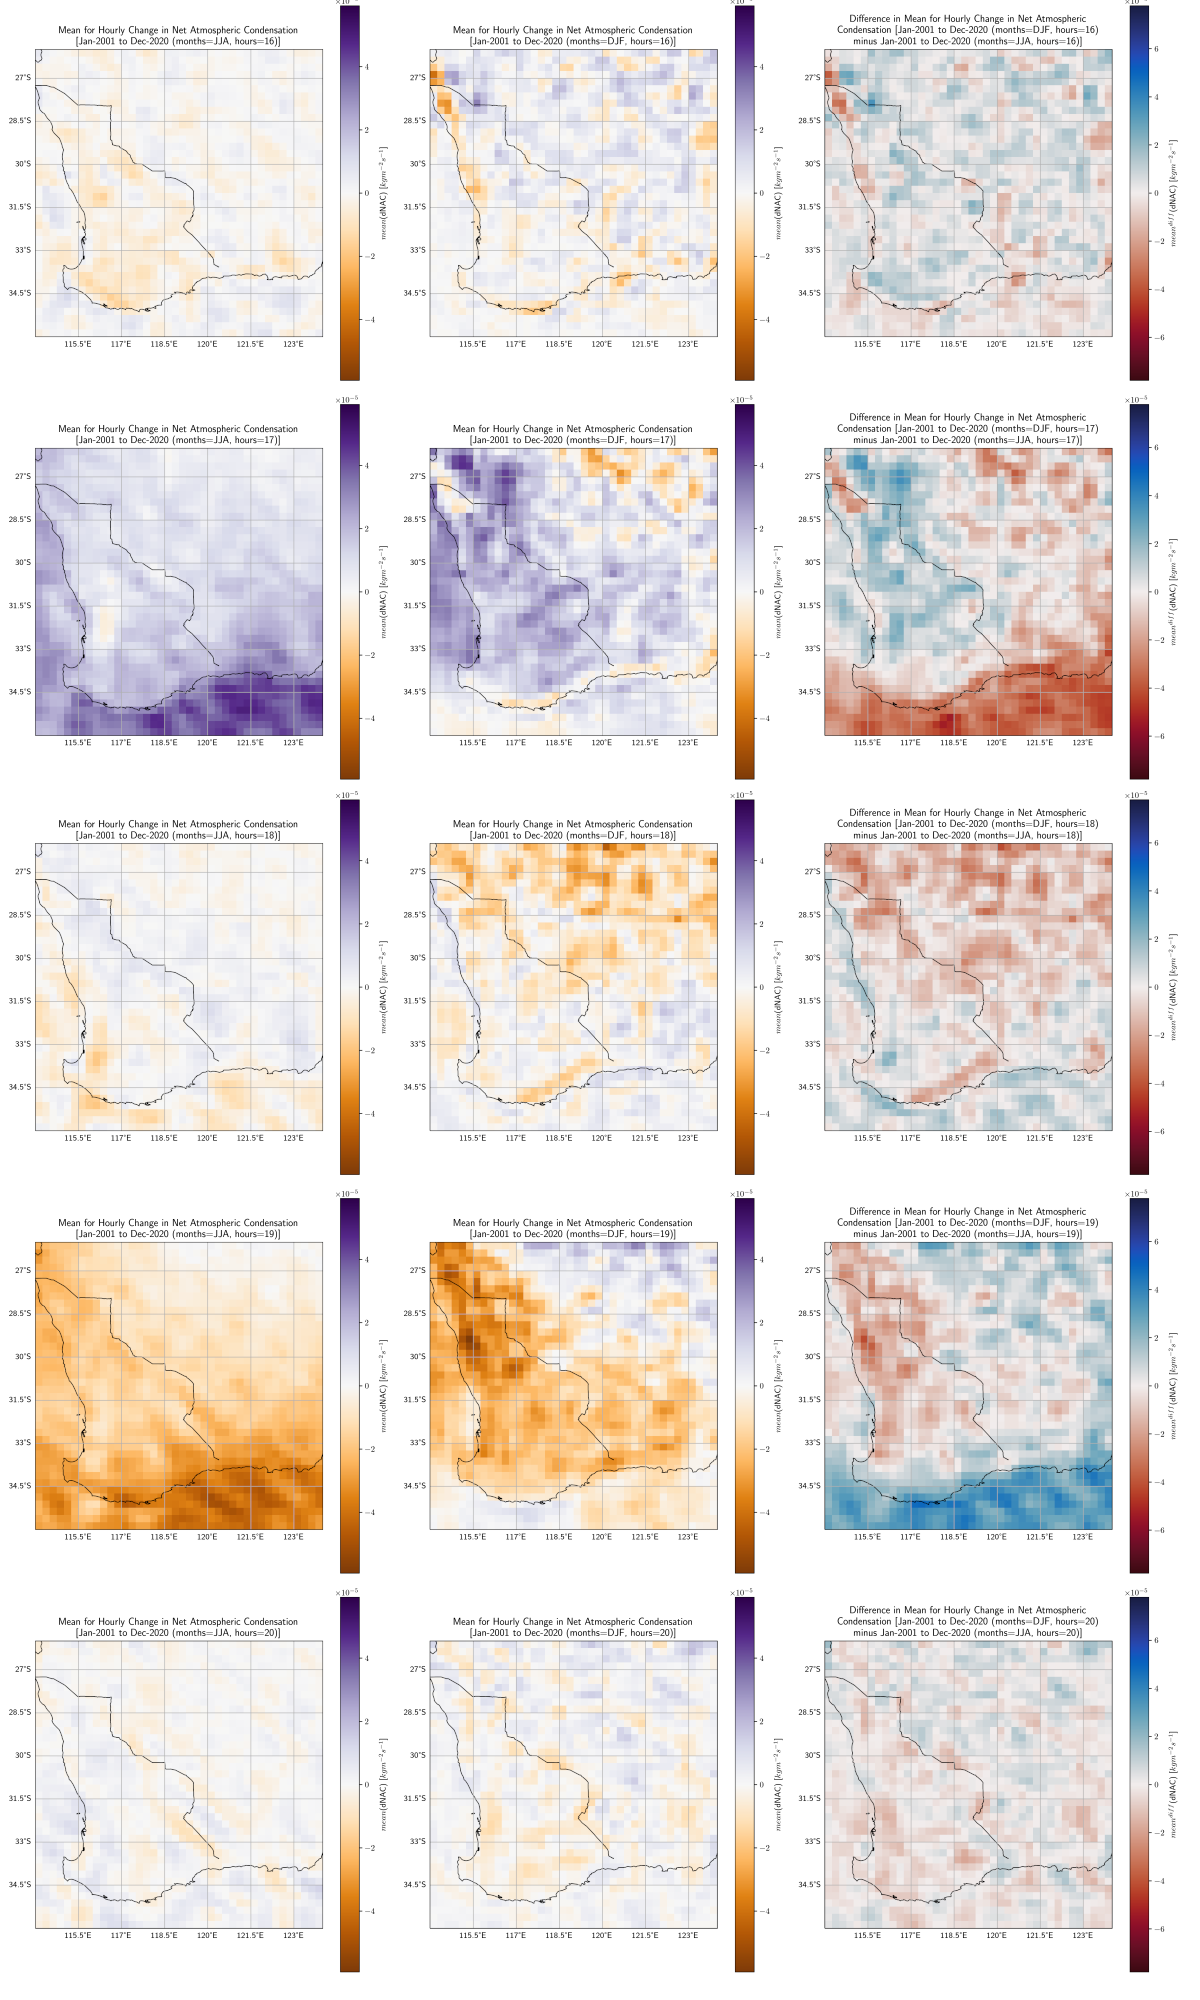
\includegraphics[width=0.75\textwidth]{wa_dnac_artefact.png}
	\caption[1600-2000 means for dNAC (artefacts)]{1600-2000 mean \ac{JJA} and \ac{DJF} values for \acs{dNAC}. 1600 and 2000 means are in line with means in remaining hours. Artefacts inherited from \ac{TCWV} assimilation cycles show opposite trends at 1700 and 1900.}
	\label{fig:wa_dnac_artefact}
\end{figure}

\subsection{Results relatively unaffected}

Figure~\ref{fig:wa_dnac_artefact} shows how this leads to unusually large \ac{dNAC} means from 1700-1900 \ac{LT}. But importantly, the increases at 1700 \ac{LT} are offset by a spatially correlated decrease of comparable magnitude at 1900 \ac{LT}. Analogous results were found between 0500-0700 \ac{LT} (not shown). So the means computed over the course of this project should be relatively unaffected. This applies even for the diurnal comparison where means were computed over a subset of hours, since daytime and nighttime hours were defined as 0800-1500 \ac{LT} and 2000-0300 \ac{LT} respectively (see Section~\ref{ssec:method_diurnal_seasonal}), which falls outside of the hours with artefacts. This does mean, however, that \ac{MDP} statistics apart from the mean (hour of maximum, hour of minimum, maximum, minimum and range) need to be interpreted with care when it comes to \ac{TCWV}, \ac{dTCWV}, \ac{NAC} and \ac{dNAC}. 

\subsection{Other affected variables}

None of the other key study variables apart from \ac{FA} were found to have similarly obvious assimilation cycle discontinuities, but \ac{FA} was only used for one result (Figure~\ref{fig:wa_stats_seasonal_2}) which was a mean over all hours of the day so results should still be relatively unaffected.

\section{Other focus regions in original project scope}
\label{sec:other_regions}

The original project scope included results for \ac{CA} and \ac{NB} but time did not allow for detailed analysis, discussion and presentation of these results. Included below is a summary for each of these regions, as well as the selected periods for the similar comparison. This may be used for future research.

\subsection{General}

\subsubsection{Periods for diurnal and seasonal comparison}

For all focus regions, the diurnal and seasonal comparisons were performed over the period from Jan-2001 to Dec-2020 (inclusive). The GLASS products derived from \ac{MODIS}, the more advanced instrument, begin around Mar-2000, with the \ac{LAI} dataset ending Dec-2021 while the \ac{FAPAR} dataset ends Dec-2020 (at the time of writing). As averages starting from Mar-2000 and ending Dec-2020 would have skewed weightings for the months of January and February, we elected to use Jan-2001 as the period start instead.

\subsubsection{Wet and dry months}

Based on historical precipitation climatology, we have selected the months representing the wet and dry seasons for each region as being:
\begin{itemize}
	\item \ac{WA}: June, July, August (JJA) and December, January, February (DJF) respectively
	\item \ac{CA}: May to October (5-6-7-8-9-10) and November to April (1-2-3-4-11-12) respectively
	\item \ac{NB}: January to June (1-2-3-4-5-6) and July to December (7-8-9-10-11-12)
\end{itemize}

\subsubsection{Daytime and nighttime hours}

The local timezones for \ac{WA}, \ac{CA} and \ac{NB} are UTC+8, UTC-6 and UTC-3 respectively\footnote{The focus region for \ac{NB} spans across 35 degrees of longitude, so it actually covers multiple local timezones and over more than 2 hours of local solar timezones (15 degrees per hour). We have selected UTC-3 here because this is close to the local solar timezone for the midpoint of this region.}. Where comparisons between daytime and nighttime hours have been made, the average values for hours from 8 am to 3 pm local time\footnote{Unless otherwise stated, all times in this report are expressed in local time, and hour endpoints are inclusive.} (8-9-10-11-12-13-14-15) have been selected as representative of daytime, while the average values for hours from 8 pm to 3 am local time (0-1-2-3-20-21-22-23) have been selected as representative of nighttime.

\subsubsection{Orography}

The orography for each focus region is displayed in Figure~\ref{fig:orog}.

\begin{figure}[!ht]
	\centering
	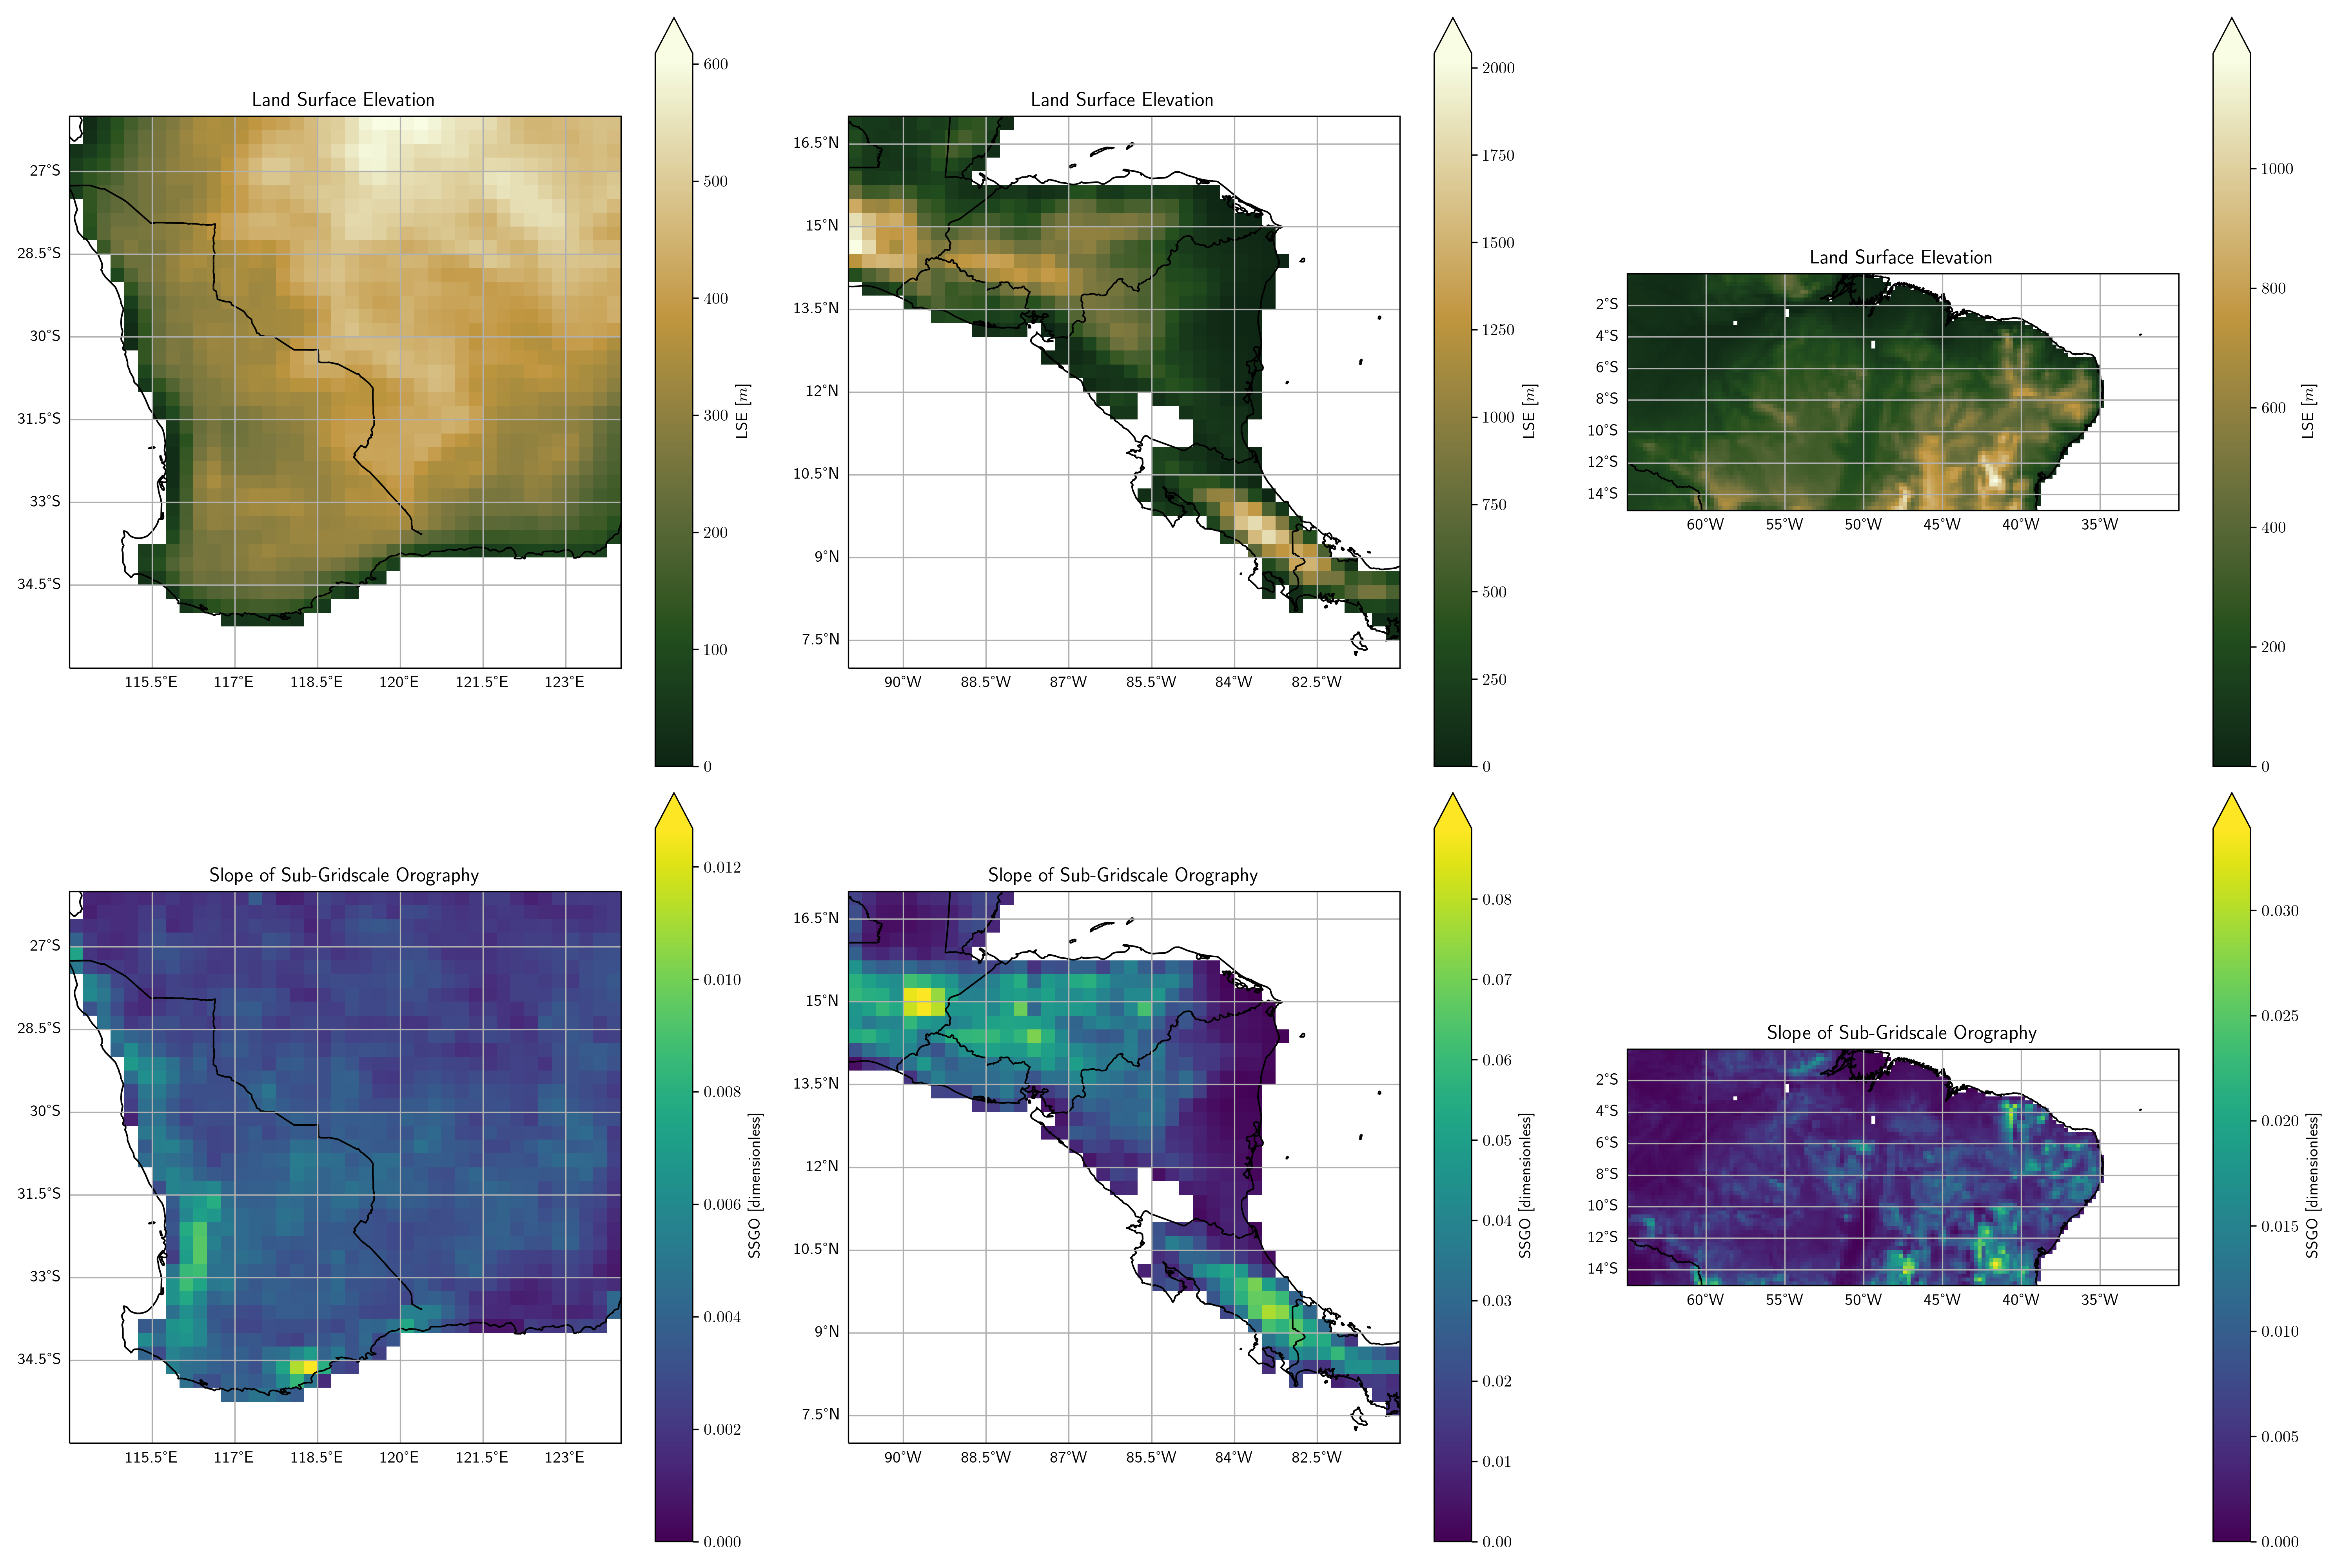
\includegraphics[width=0.9\textwidth]{orog.png}
	\caption[Orography for all focus regions]{Top row: \acf{LSE} for each region. Bottom row: \acf{SSGO} for each region. From left to right: \acl{WA}, \acl{CA}, \acl{NB}.}
	\label{fig:orog}
\end{figure}

\subsection{Central America}

\begin{figure}[!ht]
	\centering
	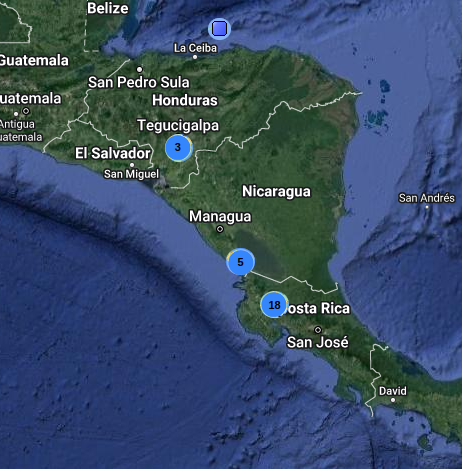
\includegraphics[width=0.75\textwidth]{maps_twp_ca}
	\caption[Central America Map]{Satellite image displaying Central America focus region from 91$^\circ$W to 81$^\circ$W longitude and 17$^\circ$S to 7$^\circ$S latitude \citep{maps_ca}. Markers indicating positions and number of wind farms have been edited on using data from \citep{twp_hd, twp_nc, twp_cr}.}
	\label{fig:maps_twp_ca}
\end{figure}

\subsubsection{Description of region}

We selected the part of \ac{CA} which runs (North to South) from El Salvador and Honduras to Nicaragua to Costa Rica (91$^\circ$W to 81$^\circ$W longitude and 17$^\circ$S to 7$^\circ$S latitude; see Figure~\ref{fig:maps_twp_ca}) because there existed spatially opposing trends in vegetation change. These countries had historically comparable rates of deforestation, but Costa Rica shifted towards reforestation due to policy changes in the 1990s whereas deforestation has continued in Honduras and Nicaragua. The western coastlines for El Salvador, Nicaragua and Costa Rica (where agriculture is concentrated) also have comparable cardinal orientations.

Being located near the equator, annual temperature variation at these locations are relatively minor. This is useful because it provides a comparison where one of the main variables affecting wind flow is relatively controlled for. Furthermore, the entire focus region is on the order of 1000 km, so synoptic weather features (which have a characteristic scale of this order) are less likely to produce contrasting effects over the different subregions.

\subsubsection{Significance of results from this region}

Wind farms are concentrated on agricultural land along the western coast where there are plans for continued development. But as in the case of \ac{WA}, the value of this focus region isn't necessarily in its direct implications for existing wind farms in the area, but in that it may yield some insights into the principles between land cover change and surface winds, which may then have broader implications for wind energy generation in general.

\subsubsection{Study periods}
\label{sssec:period_seas_ca}

\paragraph{Selected periods}

For \ac{CA}, the selected periods for the similar comparison was from Jan-2002 to Dec-2006 and from Jan-2014 to Dec-2018 (see Figure~\ref{fig:ca_ind}).

\begin{figure}[!htp]
	\centering
	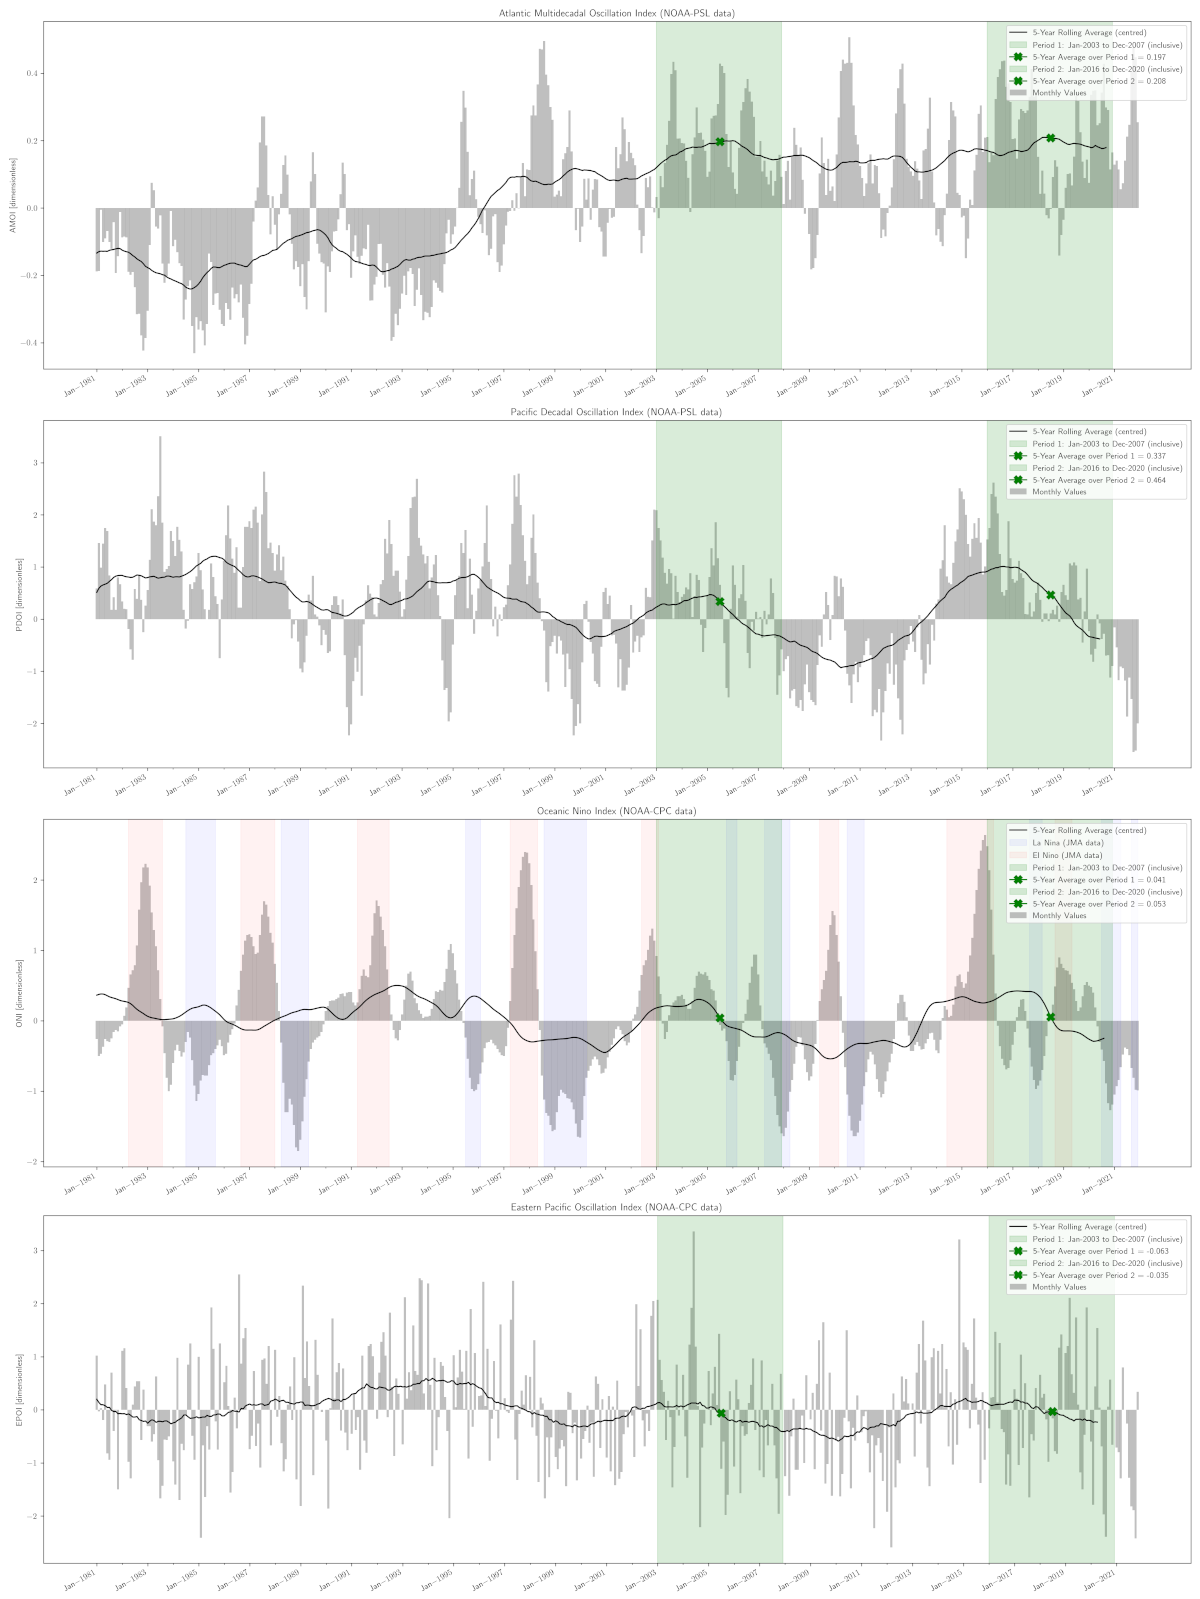
\includegraphics[width=0.9\textwidth]{ca_ind.png}
	\caption[CA's and SA's relevant climate indices for similar comparison]{\ac{NOAA} climate indices for climate drivers in \ac{CA}. Green shading highlights selected periods. Blue and red shading highlight La Nina and El Nino events respectively.}
	\label{fig:ca_ind}
\end{figure}

\paragraph{Very similar values and trends in climate indices}

The pair of Jan-2002 to Dec-2006 and Jan-2014 to Dec-2018 was deemed most appropriate since these periods had comparable averages in relevant climate indices and appear to span across the same phase of the relevant atmospheric oscillations. This was true for all of the relevant indices: \ac{AMOI}, \ac{PDOI}, \ac{ONI} (for \ac{ENSO}), and the \ac{EPOI}. The \ac{AOI} and \ac{NAOI} over these periods (not shown) also appeared to span across the same phase but had 5-year averages with slightly higher disparities (but these disparities were nevertheless small in terms of the characteristic size of the oscillations). The \ac{DMI} and the \ac{AAOI} (not shown) over these periods, on the other hand, were considerably different, but these were assumed not to be a major factor due to the distance of the Indian Ocean and Antarctica from the Americas\footnote{Significant effects due to teleconnections are theoretically possible but we have assumed this isn't the case here}.

\paragraph{Summary of ENSO events}

The similarity between these periods is particularly remarkable because even the monthly values and 5-year averages for the \ac{ONI} (which has irregular oscillations) display a similar time evolution pattern. Both periods begin with the conclusion of an El Nino event and end past halfway into an La Nina event, and fully covers another La Nina event in between. The period from Jan-2014 to Dec-2018 contains an additional El Nino event not found in the period from Jan-2002 to Dec-2006 but this appears to mostly be a technicality with the definition of an El Nino event. A look at the monthly values reveals a spike in the \ac{ONI} which could have qualified as an El Nino event under slightly relaxed definitions. Furthermore, the monthly values between the starting El Nino event and ending La Nina event are almost mirror images of each other.

\paragraph{Time difference between periods well suited for studying land cover change}

In the case of Costa Rica, although remote sensing indicates that the rate of forest cover increase here was highest during the 1990s, leaf area index data derived from the \ac{AVHRR} instrument (not shown) for this region showed considerable noise and disagreement with \ac{MODIS} (the more advanced instrument). Given these factors, this set of study periods was also desirable because it was completely contained within the \ac{MODIS} coverage period. In addition to this, a land cover classification study by \citet{marx2017} using Landsat and \ac{UAV} data in lowland Costa Rica suggested an 11-year period for a pasture to transition into secondary forest, so a 13 year difference between selected periods corresponds well with our goals for studying the effects of \ac{LCC}. The change in \ac{MLAI} between these periods is displayed in Figure~\ref{fig:ca_lai_similar}.

\begin{figure}[!ht]
	\centering
	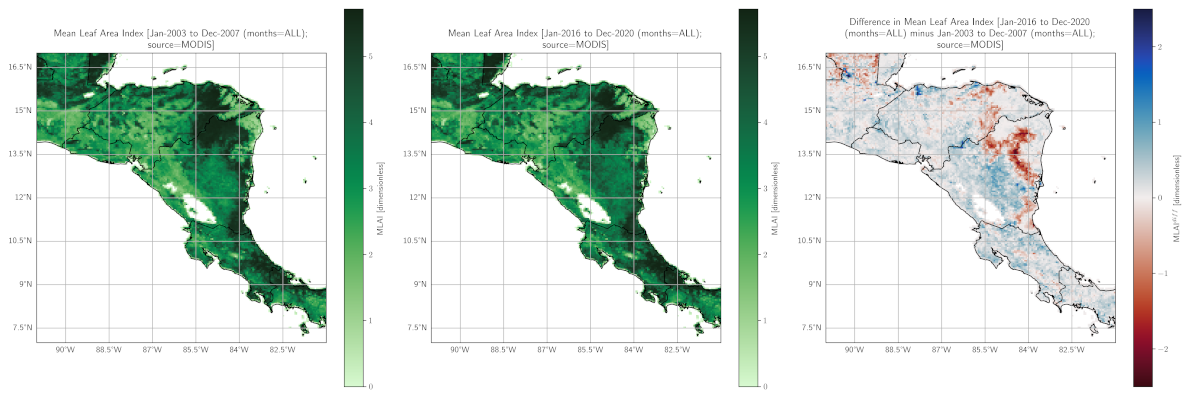
\includegraphics[width=0.9\textwidth]{ca_lai_similar.png}
	\caption[MLAI similar comparison for CA focus region]{\ac{MLAI} computed over each period in the similar comparison (left and middle), as well as the difference in these values between the two periods (right).}
	\label{fig:ca_lai_similar}
\end{figure}

\subsubsection{Land use and land cover change}

Figure~\ref{fig:lc_ca} displays trends in \ac{LULCC} at around the time of period 1 in the similar comparison.

\begin{figure}[!ht]
	\centering
	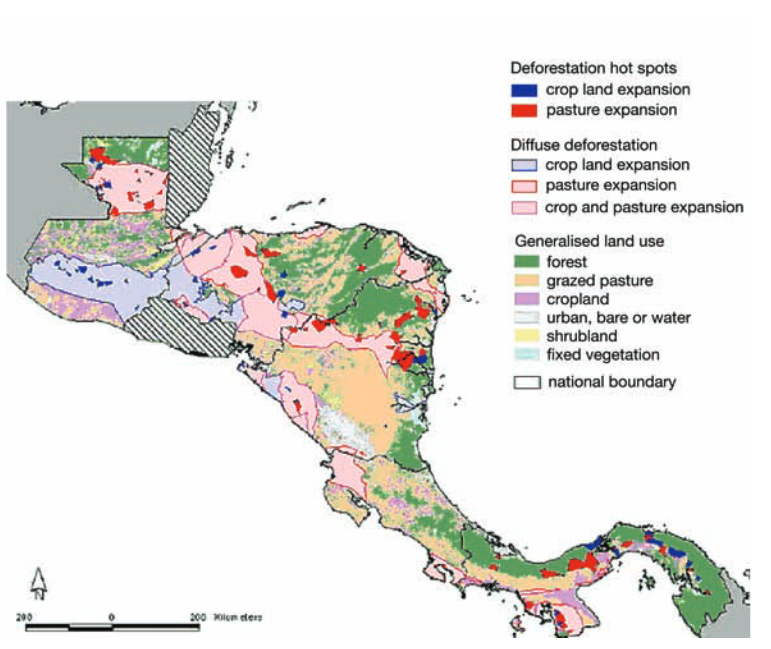
\includegraphics[width=0.75\textwidth]{lc_ca}
	\caption[Central America Land Usage]{Land usage and land cover change in Central America \citep{ipcc_2007}.}
	\label{fig:lc_ca}
\end{figure}

\subsection{Northern Brazil}

\begin{figure}[!ht]
	\centering
	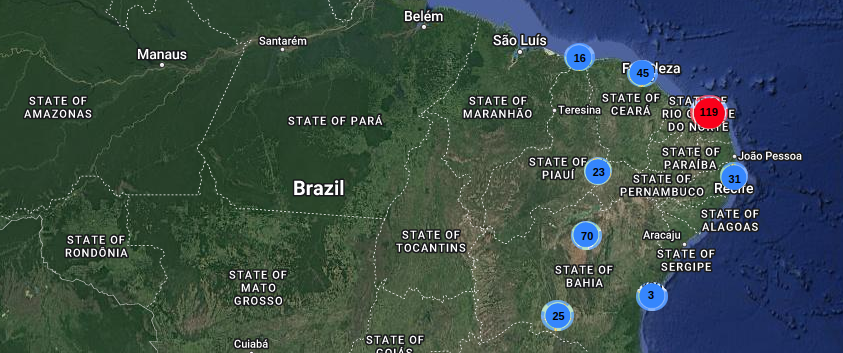
\includegraphics[width=0.75\textwidth]{maps_twp_sa}
	\caption[Northern Brazil Map]{Satellite image displaying Northern Brazil focus region from 65$^\circ$W to 30$^\circ$W longitude and 15$^\circ$S to 0$^\circ$S latitude \citep{maps_sa}. Markers indicating positions and number of wind farms have been edited on using data from \citep{twp_br}.}
	\label{fig:maps_twp_sa}
\end{figure}

\subsubsection{Description of region}

We selected the North to Northeast regions of Brazil (65$^\circ$W to 30$^\circ$W longitude and 15$^\circ$S to 0$^\circ$S latitude; see Figure~\ref{fig:maps_twp_sa}) because there has been extensive deforestation over this area and it was believed that effects resulting from \ac{LCC} here were likely to be especially pronounced. The change in \ac{MLAI} between these periods is displayed in Figure~\ref{fig:sa_lai_similar}.

\begin{figure}[!ht]
	\centering
	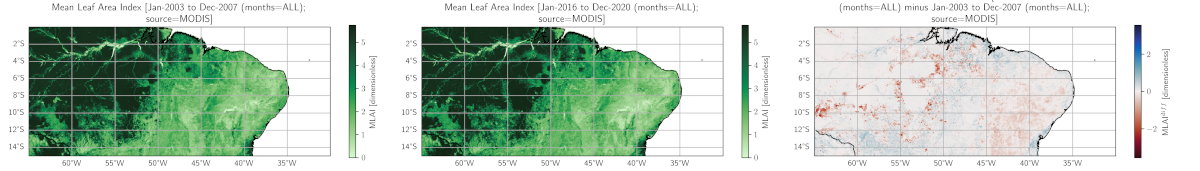
\includegraphics[width=0.9\textwidth]{sa_lai_similar.png}
	\caption[MLAI similar comparison for NB focus region]{\ac{MLAI} computed over each period in the similar comparison (left and middle), as well as the difference in these values between the two periods (right).}
	\label{fig:sa_lai_similar}
\end{figure}

\subsubsection{Significance of results from this region}

Several studies have identified large-scale changes in precipitation and moisture convergence patterns, which indirectly implicate surface wind changes. Effects here are likely to have immediate implications for energy generation due to the number of wind farms in this region (both existing and in the development pipeline\footnote{Up to 60 GW of offshore wind near the northeastern coast is in the early planning stage \citep{offshore_map}.}).

\subsubsection{Study periods}

For \ac{NB}, the selected periods for the similar comparison was from Jan-2002 to Dec-2006 and from Jan-2014 to Dec-2018 (for the same reasons highlighted in Section~\ref{sssec:period_seas_ca} for \ac{CA}.

\subsubsection{Land use and land cover change}

Figure~\ref{fig:lc_sa} displays trends in \ac{LULCC} at around the time of period 1 in the similar comparison.

\begin{figure}[!ht]
	\centering
	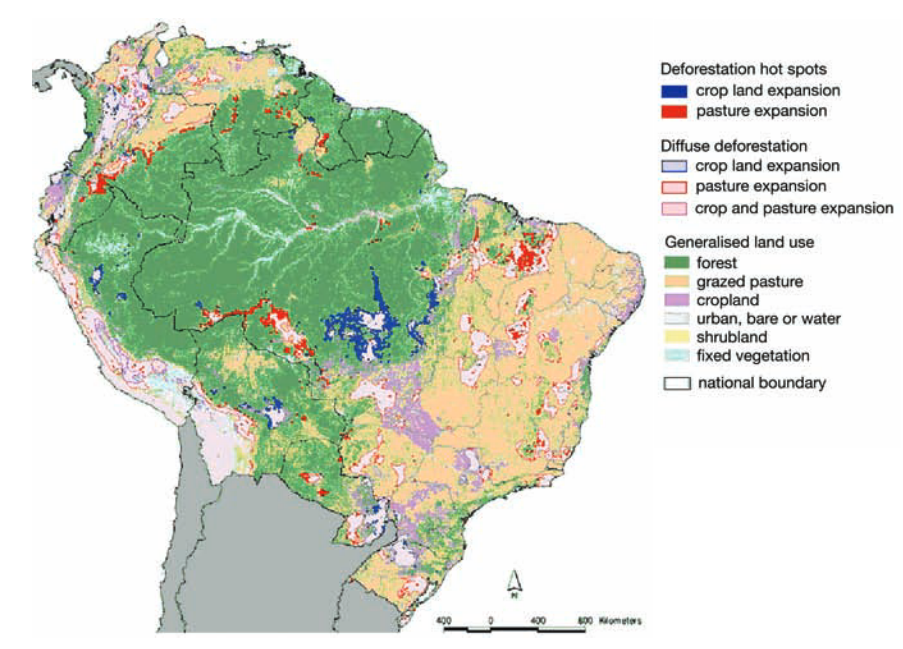
\includegraphics[width=0.75\textwidth]{lc_sa}
	\caption[Northern Brazil Land Usage]{Land usage and land cover change in Northern South America \citep{ipcc_2007}.}
	\label{fig:lc_sa}
\end{figure}